\documentclass[dvipsnames,png,border=10pt,tikz]{standalone}
\usepackage{tikz}
\usetikzlibrary{shapes.geometric} % required for the ellipse shape
\usetikzlibrary{arrows, backgrounds, calc, positioning}

\tikzset{vertex style/.style={
    draw=#1,
    thick,
    fill=#1!70,
    text=white,
    ellipse,
    minimum width=1.3cm,
    minimum height=1.3cm,
    font=\small,
    outer sep=3pt,
  },
	text style/.style={
    sloped, % the text will be parallel to the connection 
    text=black,
    font=\footnotesize,
    above
  }
}
\begin{document}
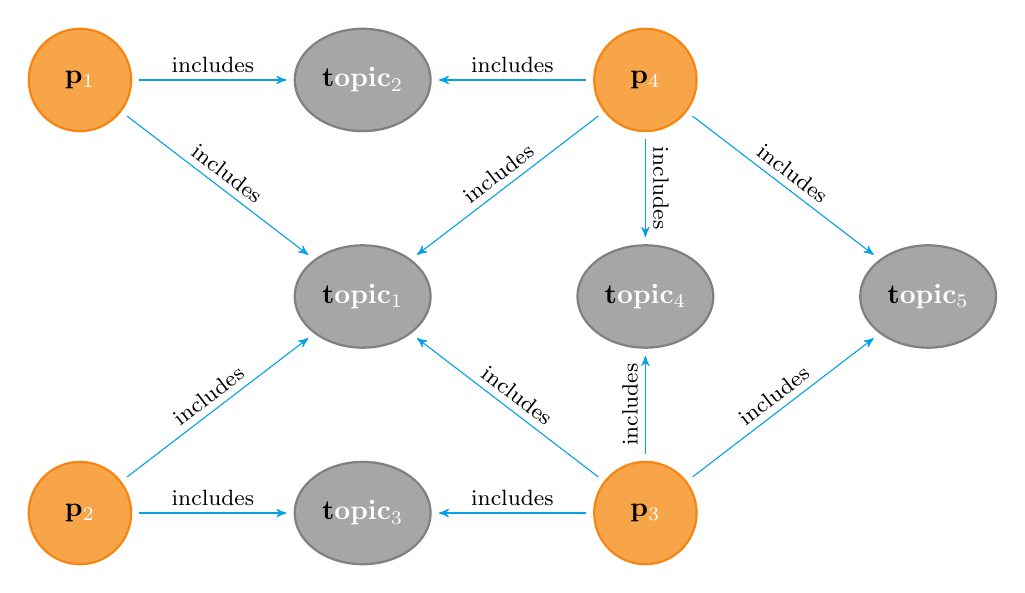
\begin{tikzpicture}[node distance=2.75cm,>=stealth']
%\node[vertex style=Turquoise] (KB) {Knowledge Base};


%\node [place,tokens=1] (w1) {};
%\node [place] (c1) [below of=w1] {};
%\node [place] (s) [below of=c1,label=above:$s\le 3$] {};
%\node [place] (c2) [below of=s] {};
%\node [place,tokens=1] (w2) [below of=c2] {};

\scriptsize
\node[vertex style=Gray, xshift=-2em] (nodeA) {\normalsize \bfseries{\textcolor{black}topic$_1$}};%NodeID: 84

\node[vertex style=Gray, right of=nodeA, xshift=3em] (nodeB) {\normalsize \bfseries{\textcolor{black}topic$_4$}};
\node[vertex style=Gray, right of=nodeB, xshift=3em] (nodeC) {\normalsize \bfseries{\textcolor{black}topic$_5$}};

\tikzset{boldstyle/.style={->,cyan!90!blue,line width=1.0pt}}
\tikzset{thinstyle/.style={->,cyan!90!blue,line width=0.5pt}}
\tikzset{tstyle/.style={<-,cyan!90!blue,line width=0.5pt}}
\tikzset{legendstyle/.style={,cyan!90!black}}

%\node[state] (A) {$A$};
%\node[state] (B) [right of=A] {$B$};
%\node[state] (C) [below of=A] {$C$};




\node[vertex style=Gray, above of=nodeA] (node2) {\normalsize \bfseries{\textcolor{black}topic$_2$}};



\node[vertex style=BurntOrange, left of=node2,xshift=-3em] (node1) {\normalsize \bfseries{\textcolor{black}p$_1$}}
edge [->,cyan!90!blue] node[text style,above]{includes} (nodeA)
edge [->,cyan!90!blue] node[text style,above]{includes} (node2);


%\path[->] (node2) [thinstyle] edge node {} (nodeA);
%\path[->] (node2) [thinstyle] edge node {} (nodeB);
 %path [->,cyan!90!blue] [mystyle] node[text style,above]{} (nodeB);

%\node[vertex style=Turquoise, above of=nodeB] (node3) {\normalsize \bfseries{125}};
%\path[->] (node3) [thinstyle] edge node {} (nodeA);
%\path[->] (node3) [thinstyle] edge node {} (nodeB);

\node[vertex style=BurntOrange, right of=node2,xshift=3em] (node4) {\normalsize \bfseries{\textcolor{black}p$_4$}}
edge [->,cyan!90!blue] node[text style,above]{includes} (nodeA)
edge [->,cyan!90!blue] node[text style,above]{includes} (node2)
edge [->,cyan!90!blue] node[text style,above]{includes} (nodeB)
edge [->,cyan!90!blue] node[text style,above]{includes} (nodeC);
%\path[->] (node4) [thinstyle] edge node {} (nodeA);
%\path[->] (node4) [thinstyle] edge node {} (nodeB);

%\node[vertex style=BurntOrange, below of=nodeA] (node7) {139}
\node[vertex style=Gray, below of=nodeA] (nodeX) {\normalsize \bfseries{\textcolor{black}topic$_3$}};
%\path[->] (nodeX) [boldstyle] edge node {} (nodeA);
%\path[->] (nodeX) [boldstyle] edge node {} (nodeB);


\node[vertex style=BurntOrange, right of=nodeX,xshift=3em] (node5) {\normalsize \bfseries{\textcolor{black}p$_3$}}
edge [->,cyan!90!blue] node[text style,above]{includes} (nodeA)
edge [->,cyan!90!blue] node[text style,above]{includes} (nodeX)
edge [->,cyan!90!blue] node[text style,above]{includes} (nodeB)
edge [->,cyan!90!blue] node[text style,above]{includes} (nodeC);
%\path[->] (node5) [thinstyle] edge node {} (nodeA);
%\path[->] (node5) [thinstyle] edge node {} (nodeB);

%\node[vertex style=Turquoise, below of=nodeB] (node6) {\normalsize \bfseries{92}};
%\path[->] (node6) [thinstyle] edge node {} (nodeA);
%\path[->] (node6) [thinstyle] edge node {} (nodeB);



%\node[vertex style=Maroon, left of=nodeA,xshift=-5.5em,label=below:eclipse/rdf4j] (node8) {\normalsize \bfseries{992}};
%\path[-] (node8) [tstyle] edge node {} (node1);
\node[vertex style=BurntOrange, left of=nodeX,xshift=-3em] (node9) {\normalsize \bfseries{\textcolor{black}p$_2$}}
%\node[vertex style=Turquoise, below left of=nodeA,xshift=-3em] (node9) {\bfseries{p$_2$}}
edge [->,cyan!90!blue] node[text style,above]{includes} (nodeA)
edge [->,cyan!90!blue] node[text style,above]{includes} (nodeX);

% edge [->,cyan!90!blue] node[text style,above]{} (nodeA)
% edge [->,cyan!90!blue] node[text style,above]{} (node8);

%\node[vertex style=BurntOrange, below right of=node7,label=right:$\times 10$  nodes,label=below:$(153;155;163;164;171;173;176;196;201;210)$] (nodeX) {...}
 %edge [->,cyan!90!blue] node[text style,above]{} (nodeA)
 %edge [->,cyan!90!blue] node[text style,above]{} (nodeB);

%\node[vertex style=BurntOrange, below left of=nodeA,xshift=-1em] (node8) {151}
 %edge [->,cyan!90!blue] node[text style,above]{} (nodeA)
 %edge [->,cyan!90!blue] node[text style,above]{} (nodeB);


% \node[text width=3cm] at (-5,3) {\normalsize \bfseries{Legend}};
%
% \draw[boldstyle, yshift=-1em]
%  (current bounding  box.north west)
%  ++(0, -3em) -- ++(2em, 0)
%  node[right,black] {\normalsize isUsedBy};
%
%  \draw[thinstyle, yshift=-1em]
% (current bounding  box.north west)
% ++(0, -2em) -- ++(2em, 0)
% node[right,black] {\normalsize stars};
% 
 

 

%\tikzset{boldstyle/.style={->,cyan!90!blue,line width=1.0pt}}
%\tikzset{thinstyle/.style={->,cyan!90!blue,line width=0.5pt}}
%\tikzset{bstyle/.style={<-,cyan!90!blue,line width=1.0pt}}


%\node [place] (s) [above of=node4,label=above:$s\le 3$] {};


\end{tikzpicture}

\end{document}
